% paper.tex — arXiv preprint source, generated 2026-10-13 from 04_manuscript.md
% Build: any LaTeX toolchain that runs BibTeX (pdflatex -> bibtex -> pdflatex x2),
%        or `tectonic paper.tex` in this directory (requires references.bib + figures/).
% For arXiv upload: include the generated paper.bbl (arXiv does not run BibTeX).
%
% NOTE(submission): self-description is "structured evidence audit" (original
% research: new coding instrument + 44-record dataset + statistical analysis),
% NOT "position paper" — see 05_submission_package.md §1.3 (arXiv cs policy of
% 2025-10-31 restricting review/position papers).

\documentclass[10pt]{article}

\usepackage[margin=1in]{geometry}
\usepackage[T1]{fontenc}
\usepackage[utf8]{inputenc}
\usepackage{newtxtext,newtxmath}
\usepackage{microtype}
\setlength{\emergencystretch}{2em}
\usepackage{graphicx}
\graphicspath{{figures/}}
\usepackage{booktabs}
\usepackage{array}
\usepackage[numbers,sort&compress]{natbib}
\usepackage{xcolor}
\usepackage[colorlinks=true,linkcolor=blue!60!black,citecolor=blue!60!black,urlcolor=blue!60!black]{hyperref}
\urlstyle{same}

\newcommand{\level}[1]{\textbf{#1}}

\title{\textbf{Success Provides Direction, Failure Provides Precision:\\
A Structured Audit of Failure Data in LLM Training}}

\author{Yu Yugui\\
Yu Yugui Strategy Lab\\
\texttt{they4897@gmail.com}
% TODO(user): add ORCID before arXiv submission
}
\date{October 13, 2026}

\begin{document}
\maketitle

\begin{abstract}
\noindent A durable intuition from human learning---students keep error notebooks because mistakes, once explained, sharpen far more than repeated successes---has no systematic counterpart in large language model (LLM) training data. We formalize this intuition as a testable claim: success examples provide direction, while attributed failure examples provide precision, because each explained failure contracts the space of plausible policies. To measure how far current practice stands from this ideal, we audited how training pipelines actually treat failure data, coding 33 evidence units (28 open-source datasets and recipes; five flagship pipelines released in autumn 2026) with a five-level lifecycle codebook---L0 discard, L1 shadow, L2 transient, L3 component, L4 first-class---plus six sub-dimensions. The L4 tier, failure data combining error annotation, causal attribution, and reflective correction at scale under a public methodology, is vacant: 0/33 units. Mainstream 2023--25 recipes top out at transient gradients: 0/15 reach L3, and all seven SFT-stage units are pure L0. By contrast, four of five 2026 flagships operate explicit failure-data components (cohort median L3), and the failure-signal vehicle is migrating from preference pairs (6/15 mainstream units) to RL environments and audit loops (0/14 flagship mechanisms). Failure data with all three elements exists in exactly one unit (1/33). We argue that, within the audited disclosure layer, failure data is an unoccupied high ground, and we specify the components required to make it a first-class citizen.
\end{abstract}

\medskip
\noindent\textbf{Keywords:} failure data; learning from mistakes; error-annotated data; post-training; RLVR; data curation

\section{Introduction}

Human learners have long institutionalized the study of failure: the error notebook, in which a student records each mistake, diagnoses its cause, and writes out the corrected reasoning, is a standard artifact of mathematics education in China and elsewhere. In July 2026, the vice president of Fudan University, Yungang Jiang, publicly argued at the World Artificial Intelligence Conference that failure data is as important for model capability as success data, explicitly invoking the error-notebook metaphor for foundation-model corpus construction \cite{waic2026}. The metaphor resonates because it names something the field practices in private and discards in public: every reinforcement learning (RL) run generates failures, every verifier flags them, and almost none of them survive as training assets.

This paper defends a precise version of that intuition.\label{sec:intro-arg} Our claim is that \textbf{success provides direction, while failure provides precision}. In Bayesian terms, a correct demonstration confirms that some policy works; an \emph{attributed} failure eliminates a region of the hypothesis space. Accumulated, diverse, well-explained failures contract the posterior toward the correct policy in a way that additional successes cannot replicate, since successes in the same region are largely redundant. The claim comes with quality caveats that we carry throughout: failures must be diverse and information-dense rather than homogeneous; they must be detoxified, since fake successes such as reward hacking are actively harmful; and coverage of failure modes, not any fixed success-to-failure ratio, is the operative variable.

The intuition has non-trivial cognitive antecedents, which we invoke as motivation rather than proof. The description--experience gap shows that judgments formed from sampled experience, including experienced losses, systematically differ from those formed from described probabilities, suggesting that experienced outcomes carry signal that descriptions do not \cite{hertwig2009}. Studies of the Iowa Gambling Task indicate that losses can be encoded implicitly, as somatic markers that precede conscious insight, and still guide choice \cite{bechara2005}. We do not claim these results transfer to gradient descent; they motivate the hypothesis that explained failures carry information that successes do not.

Why does this matter now? Because generalization and calibration are currently among the weakest dimensions of frontier models, and the evidence points at training-data practice. Reinforcement learning with verifiable rewards (RLVR) appears to reweight existing capability rather than expand it: pass@1 rises while pass@$k$ at large $k$ does not surpass the base model \cite{yue2025rlvr}. Hallucination has been argued to be a structural property of the pretraining--posttraining interface, with evaluations that reward confident guessing reinforcing miscalibration \cite{kalai2025halluc}. Post-training itself damages calibration, with aligned models measurably more overconfident than their pretrained checkpoints \cite{he2023calibration}, and RL-style objectives (PPO, GRPO, DPO) inducing overconfidence through reward exploitation \cite{xie2026know}. Failure-driven learning is a candidate training signal for precisely these dimensions---learning where the boundary of one's competence lies---and controlled evidence already exists: fine-tuning on machine-annotated error--correction pairs lifted LLaMA-2-70B to 83.5\% on GSM8K, surpassing GPT-4 at the time \cite{an2023lema}, and process reflection supervision turned a collapsing tool-use RL run into a $+22.25$-point gain with nonzero scores on double-unseen out-of-distribution scenarios where an SFT baseline scored exactly zero \cite{hao2026prs}.

What is missing is an account of practice. Scattered technical-report disclosures---rejection sampling that discards failed trajectories, preference pairs whose rejected side silently carries failure, RL environments that replay observed weaknesses---have never been systematically compared, for want of a shared vocabulary for ``how this pipeline treats failure data.'' That gap, between proven methodology and adopted methodology, is our subject.

We contribute four things:

\begin{itemize}
\item \textbf{A lifecycle codebook} that grades how a training pipeline treats failure data on an ordinal scale from L0 (discarded) to L4 (first-class), with six orthogonal sub-dimensions (Section~\ref{sec:codebook}), making ``what happens to failures'' comparable across papers and vendors for the first time.
\item \textbf{A two-layer audit} applying this codebook to 33 evidence units---28 open-source datasets and mainstream recipes, and five 2026 flagship pipelines---yielding 44 mechanism-level coding records anchored to primary sources (Section~\ref{sec:method}).
\item \textbf{A quantified generational shift}: mainstream 2023--25 recipes contain no unit at L3 or above (0/15) while four of five autumn-2026 flagships operate explicit failure components, with the failure-signal vehicle migrating from preference pairs to RL environments and audit loops (Section~\ref{sec:results}).
\item \textbf{A roadmap} specifying the components---tripartite data schema, collection protocols, toxicity cleaning, verifier-dependence handling, open corpora, and evaluation---that first-class failure data still requires, with falsifiable monitoring indicators (Section~\ref{sec:roadmap}).
\end{itemize}

The paper proceeds as follows. Section~\ref{sec:background} organizes prior work into five families of failure signals plus the 2026 industry disclosure line, and states the gap. Section~\ref{sec:codebook} presents the codebook. Section~\ref{sec:method} details the audit method. Section~\ref{sec:results} reports results against our four research questions. Section~\ref{sec:discussion} discusses implications and limitations. Section~\ref{sec:roadmap} gives the roadmap; Section~\ref{sec:conclusion} concludes.

\section{Background: Five Families of Failure Signals}\label{sec:background}

We organize prior work not by paper but by the \emph{role the failure signal plays in training}. Five families exist, plus a 2026 industry disclosure line; each holds a partial proof of the value of failure data, and none completes it.

\subsection{Contrastive negatives: failure as decision boundary}

Negative sampling is the oldest systematic use of ``what is wrong.'' The survey literature reports that the hardest negatives carry the most information gain, with as little as 5\% of the hardest negatives supporting high-precision contrastive learning \cite{yang2024negsampling}. Theory confirms that more negatives do not necessarily hurt downstream generalization \cite{awasthi2022negative}, and negative-dominant objectives---upweighting negatives under imbalance---achieve the best Friedman ranks in domain-generalization studies (4.80, best among compared methods) \cite{cao2026ndcl}. This family demonstrates that failure signals can be the \emph{dominant} learning signal, but it has remained in representation learning and never entered LLM post-training.

\subsection{Process-supervision error annotation: failure as step-level label}

A second family annotates \emph{where} reasoning fails. PRM800K provides 800,000 step-level human ratings on math solutions, with erroneous steps explicitly marked \cite{lightman2023verify}; Math-Shepherd derives step-correctness probabilities automatically at a scale of roughly 400,000 samples \cite{wang2024mathshepherd}. The evaluation side extends this: ProcessBench tests whether models can locate the first erroneous step among 3,400 solutions \cite{zheng2024processbench}, and PRMBench probes six error types across about 11,000 samples \cite{song2025prmbench}. This family solves localization but produces labels, not teaching material.

\subsection{Error--correction fine-tuning: failure as teaching material}

The family closest to the error notebook converts failures into lessons. LEMA fine-tunes on erroneous solutions paired with GPT-4-generated identification and correction of the mistakes---roughly 24k--50k pairs---and shows that such error--correction data is not homogeneous with chain-of-thought data, with larger gains for weaker models \cite{an2023lema}. Process Reflection Supervision (PRS) is, to our knowledge, the strongest recent demonstration: it diagnoses why multi-step tool-use RL collapses, then has an auxiliary analyzer (gpt-5-mini) generate root-cause analyses and improvement plans for failed trajectories, trained jointly with an SFT loss; on BFCL-V3, PRS reaches an average of 25.75 versus 3.50 for vanilla GRPO ($+22.25$ points, with GRPO collapsing to zero in some settings), and on ACEBench scenarios unseen in both content and format, PRS scores 12.00 where the SFT baseline scores 0.00---the hardest existing evidence that reflective failure data produces \emph{generalization rather than memorization} \cite{hao2026prs}. In embodied domains, AHA trains a vision--language model to detect and reason over robotic manipulation failures \cite{duan2024aha}, and Foresight targets failure detection in long-horizon manipulation \cite{zhang2026foresight}; both stop at detection. The family's limitation is scale and adoption: tens of thousands of pairs, no mainstream recipe.

\subsection{The rejected side of preference pairs: failure as relative signal}

In preference alignment, failure survives only as the \emph{rejected} member of a chosen--rejected pair, without independent semantics. Llama 3 constructs pairs by score gaps \cite{grattafiori2024llama3}; Qwen3 routes verifier-rejected responses to the rejected side or discards them \cite{qwen2025qwen3}; Tulu 3 builds roughly 270,000 on-policy preference prompts \cite{lambert2025tulu3}; HH-RLHF contributes about 170,000 human-written pairs \cite{anthropic2022hhrlhf}; UltraFeedback couples low scores with per-aspect critiques \cite{openbmb2023ultrafeedback}; SmolLM2 performs DPO over low-rated responses \cite{hftb2024smoltalk}. MIPO, the mixed-integer preference objective in GLM-4.5, graded negative-sample strength in mixing---the closest the preference era came to systematic negative-signal retention \cite{zai2025glm45}. Our audit codes MIPO as L1 (Section~\ref{sec:results}); its retirement in GLM 5.x (Section~\ref{sec:results}) marks the vehicle's decline. NPO formalizes unlearning as negative preference optimization, repurposing ``forget'' sets as negatives \cite{zhang2024npo}. Across the family, failure never appears as an absolute, teachable signal.

\subsection{RL failure signals: failure as gradient component}

In RL, failed rollouts contribute negative advantage and are then discarded---used transiently, never released. This is the GRPO pattern in DeepSeek-R1 \cite{deepseek2025r1}. More telling, discarding has been institutionalized at the algorithm level: DAPO's dynamic sampling explicitly removes prompt groups in which \emph{all} rollouts fail, framing zero-gradient groups as compute waste \cite{yu2025dapo}. On the agent side, ETO pairs failed and successful trajectories for contrastive training \cite{song2024eto}, and UltraInteract packs error-containing tree trajectories with reflections into preference pairs \cite{yuan2024ultrainteract}. The family shows failure as a live but unarchived signal.

\subsection{The 2026 industry disclosure line}

Between August and October 2026, first-party disclosures of five flagship pipelines revealed explicit failure-data mechanisms: GPT-6 Astra routes failure signals to monitoring and evaluation rather than training data, with RL penalties on cheating as the only training-side use \cite{openai2026gpt6}; Claude Opus 5.5's Alignment Intelligence Report drives training improvements from more than 7,200 collected agent failure scenarios, within the alignment domain \cite{anthropic2026claude}; GLM-5.3 retains erroneous trajectory segments under loss masks and selects RL tasks that the previous generation persistently fails \cite{zai2026glm5}; MiMo-V2.6 synthesizes reflection-and-revision training samples from real reward-hacking failures \cite{xiaomi2026mimo}; and DeepSeek-V4.1-Flash collects employee-submitted failure cases at scale and replays them through targeted RL \cite{deepseek2026v41}. Policy-side attention exists \cite{waic2026}, but the corpus establishment has not followed: the Chinese foundational corpus release of September 2026 contains no failure-corpus track \cite{cac2026corpus}.

\subsection{The gap}

Each family holds a piece of the proof: contrastive negatives establish that failure can dominate learning (but only in representation space); process supervision establishes localization (but not correction); error--correction fine-tuning establishes teaching value (but at $10^4$--$10^5$ scale, outside mainstream recipes); the rejected side institutionalizes failure in its weakest form; RL uses failure transiently and discards it. The 2026 disclosure line shows industrial components arriving, unnamed and unreleased. No family, recipe, or vendor---as of 2026-10-13 and within disclosed practice---treats failure data combining error localization, causal attribution, and reflective correction as a first-class, scaled, public training methodology. The audit below measures exactly this gap.

\section{A Lifecycle Codebook for Failure Data}\label{sec:codebook}

The \textbf{unit of coding} is a failure-handling mechanism in a training pipeline or dataset, anchored to a citable primary source; a unit with multiple mechanisms (e.g., DAPO) receives one mechanism record per mechanism, and its main code is the highest level among them. By \emph{failure} we mean any sample or trajectory that the system itself judges erroneous, unverified, or rejected. The \textbf{main code} grades the unit on an ordinal lifecycle scale, with criteria in universal-quantifier form (all listed criteria must hold):

\begin{itemize}
\item \level{L0 --- Discard.} Failed trajectories are filtered before training (verification, rejection sampling, or filtered release); the release contains no failure instances; no failure processing exists. \emph{Example:} DeepSeek-R1's third-stage rejection sampling keeps only correct, language-consistent, high-quality trajectories \cite{deepseek2025r1}. \emph{Boundary:} OpenMathInstruct-2 ships an \texttt{expected\_answer} field that enables right/wrong judgment; a field enabling judgment is not a retained failure instance, so the unit codes L0 \cite{nvidia2024omi2}.
\item \level{L1 --- Shadow.} Failure exists only as the rejected side of preference pairs, with no independent error semantics, and is not separately released. \emph{Example:} HH-RLHF pairs \cite{anthropic2022hhrlhf}. \emph{Boundary:} UltraInteract's rejected side carries explicit reflection text, which satisfies an L3 criterion; the unit is coded multi-level L1+L3 with main code L3 \cite{yuan2024ultrainteract}.
\item \level{L2 --- Transient.} Failed rollouts contribute gradient (negative advantage or penalty) during training, are discarded afterward, and are never released. \emph{Example:} GRPO's failed rollouts \cite{deepseek2025r1}. \emph{Boundary:} DAPO exhibits in-group negative advantage (L2) \emph{and} explicit removal of all-failure groups (an L0 feature); the mechanisms are split, and the unit's main code is L2 \cite{yu2025dapo}.
\item \level{L3 --- Component.} Failure is explicitly retained or processed into a recognizable component---loss masks, audit labels, replay environments, synthetic correction samples, or reflection reports---but the component is localized or domain-limited, and is not released or theorized as public methodology. \emph{Example:} GLM-5.3's error-segment masking \cite{zai2026glm5}. \emph{Boundary:} OpenR1-Math-Raw releases roughly one million raw trajectories including unverified ones---the highest-openness L3 in our corpus---but the three elements are incomplete, so it does not reach L4 \cite{openr12025mathraw}.
\item \level{L4 --- First-class.} Error annotation, causal attribution, and reflective correction are all present; the data operates at scale ($10^{5+}$ samples or as an industrial-pipeline core); it is explicitly named and theorized as methodology; and the data or methodology is public. The codebook anticipated that L4 would be empty; the vacancy, once confirmed, is itself a finding rather than a coding failure.
\item \level{No-disclosure.} For flagship pipelines, absence of failure-data disclosure is coded as \emph{no-disclosure}, not L0: L0 requires an explicit statement of filtering. In the final corpus, zero units fell into this category---all 33 units could be leveled from the locked corpus.
\end{itemize}

Six \textbf{sub-dimensions} are coded independently at the highest verifiable form: error granularity (none / trajectory / step / causal), attribution (none / binary model-versus-environment / root-cause), reflection (none / correction-pair / full reflective report), domain (capability / alignment), openness (released / not-released), and vehicle (static dataset / preference pair / RL environment / audit loop). The first three---localize, attribute, reflect---constitute the \emph{three elements} whose joint presence defines the error-notebook form. Figure~\ref{fig:lifecycle} renders the framework with unit counts; the L4 tier is drawn vacant.

\begin{figure}[t]
\centering
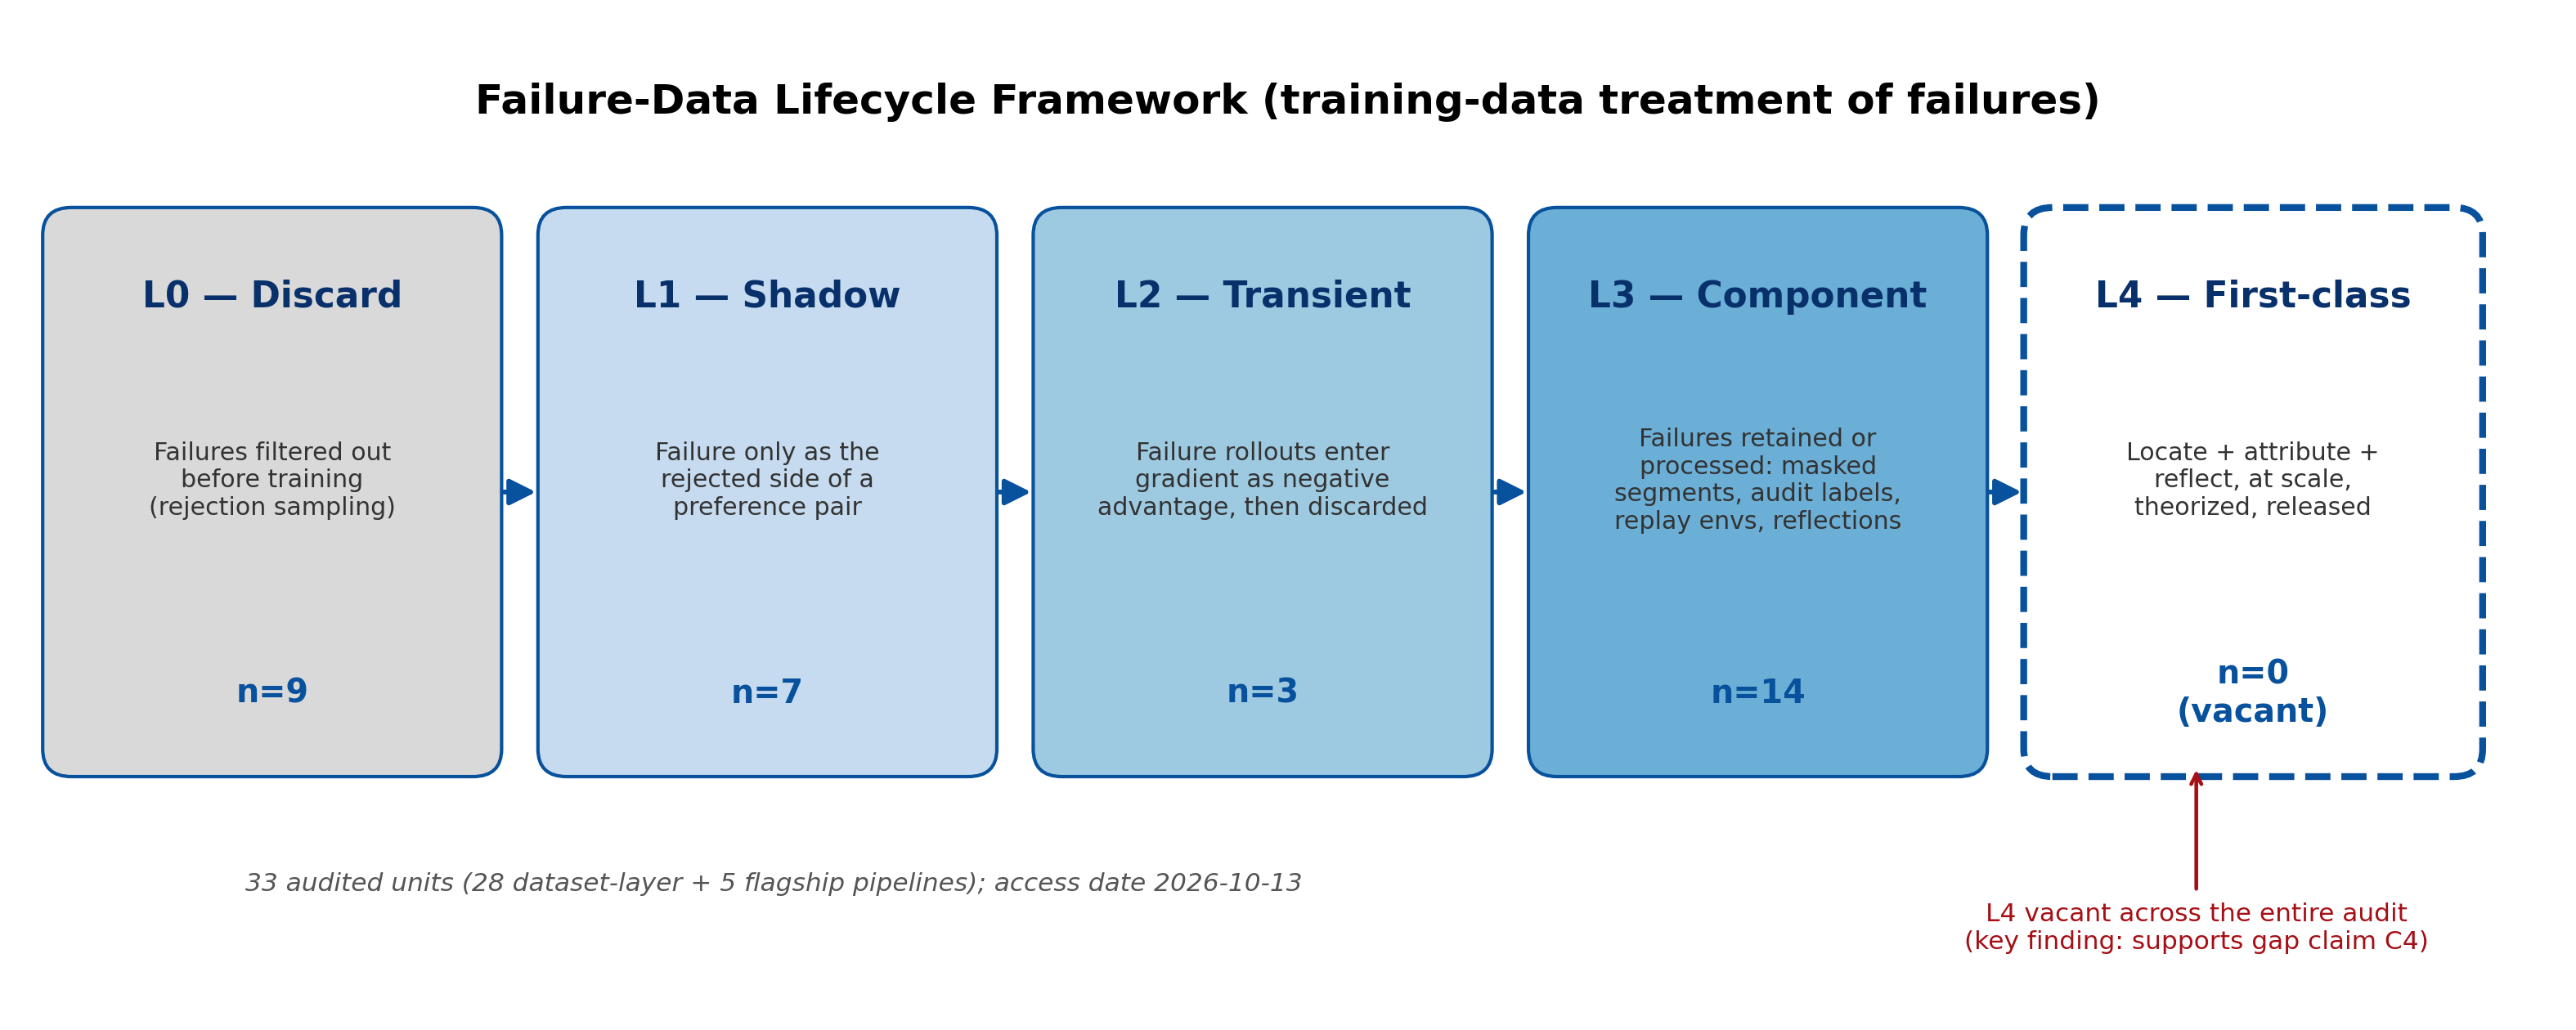
\includegraphics[width=0.95\textwidth]{fig1_lifecycle_framework.png}
\caption{The failure-data lifecycle framework (L0--L4). Unit counts from the audit of 33 units (28 dataset-layer + 5 flagship pipelines); the L4 tier is vacant across the entire audit---itself the paper's key finding.}
\label{fig:lifecycle}
\end{figure}

Two coding disciplines apply throughout. First, L0--L4 is ordinal: we report frequencies and medians, never means. Second, ``not disclosed'' never implies ``does not exist'': disclosure asymmetry is treated as a validity threat, not evidence (Section~\ref{sec:limitations}).

\section{Audit Method}\label{sec:method}

\subsection{Design and corpora}

The study is a document audit of publicly available sources; it involves no human subjects. Evidence was assembled in two layers, locked as audit-v1.0 on 2026-10-13.

\textbf{Corpus A (dataset layer, $n{=}28$)} covers open training recipes and datasets across five stages, each anchored to a primary source: pre-training---Dolma \cite{ai22024dolma}, FineWeb \cite{hf2024fineweb}; SFT/distillation---DeepSeek-R1 \cite{deepseek2025r1}, Llama 2 \cite{touvron2023llama2}, Llama 3 \cite{grattafiori2024llama3}, OpenR1-Math-220k \cite{hf2025openr1}, Bespoke-Stratos \cite{bespokelabs2025stratos}, OpenMathReasoning \cite{nvidia2025omr}, OpenMathInstruct-2 \cite{nvidia2024omi2}; preference alignment---Llama 3 DPO \cite{grattafiori2024llama3}, Qwen3 \cite{qwen2025qwen3}, Tulu 3 \cite{lambert2025tulu3}, HH-RLHF \cite{anthropic2022hhrlhf}, SmolLM2 \cite{hftb2024smoltalk}, GLM-4.5 MIPO \cite{zai2025glm45}; RL---GRPO as implemented in R1 \cite{deepseek2025r1}, DAPO \cite{yu2025dapo}; and academic exceptions---PRM800K \cite{lightman2023verify}, Math-Shepherd \cite{wang2024mathshepherd}, LEMA \cite{an2023lema}, ETO \cite{song2024eto}, UltraInteract \cite{yuan2024ultrainteract}, UltraFeedback \cite{openbmb2023ultrafeedback}, ProcessBench \cite{zheng2024processbench}, PRMBench \cite{song2025prmbench}, OpenR1-Math-Raw \cite{openr12025mathraw}, NPO's unlearning sets \cite{zhang2024npo}, and SPAR f26 \cite{spar2026f26}. Inclusion required a verifiable primary document (paper, official data card, or official repository), community adoption or methodological representativeness, and disclosure no later than 2026-10-13. Units supported only by media reports were excluded; one widely circulated embodied failure-analysis dataset could not be located in primary sources after multiple targeted searches and was removed from the evidence chain entirely---embodied failure reasoning is instead cited through verifiable work \cite{duan2024aha}.

\textbf{Corpus B (pipeline layer, $n{=}5$)} covers flagships released after Jiang's July 2026 remarks, each anchored to first-party documentation: GPT-6 Astra's system card \cite{openai2026gpt6}, Claude Opus 5.5's system materials \cite{anthropic2026claude}, the GLM-5 technical report (anchor for GLM-5.3) \cite{zai2026glm5}, MiMo-V2.6 \cite{xiaomi2026mimo}, and DeepSeek-V4.1-Flash \cite{deepseek2026v41}. This is saturation purposive sampling---the five are the recognized first tier of closed and open flagships---not probability sampling; conclusions are accordingly limited to \emph{disclosed practice}. A literature corpus (the five families above) and an arXiv re-check over August--October 2026 complete the materials.

\subsection{Procedure}

Coding followed the pipeline: locate $\rightarrow$ include/exclude $\rightarrow$ primary-source verification $\rightarrow$ mechanism-level coding $\rightarrow$ reliability recheck $\rightarrow$ data lock. Each of the 44 mechanism records (30 in Corpus A, 14 in Corpus B) carries a verbatim or excerpt-level quote with section anchor, source tier, confidence rating, and conflict-rule citations. Five conflict rules govern judgments: multi-mechanism units take the highest level as main code (CR1); primary sources override secondhand ones (CR2); versions of the same vendor are split into separate records (CR3); undecidable criteria yield low confidence and never inference (CR4); and no-disclosure is never coded L0 (CR5). For Corpus B, every code at L2 or above is anchored to a verbatim quote of at most 50 words.

\subsection{Verification corrections}

Because our upstream evidence chain contained two propagating errors, we enforced a verification gate on all load-bearing numbers. PRS is cited from the verified primary source (arXiv:2606.26027), with the analyzer model corrected to gpt-5-mini and gains reported as $+22.25$ points (25.75 versus 3.50), never converted into a ratio multiple \cite{hao2026prs}. DAPO is cited under its correct identifier (arXiv:2503.14476) \cite{yu2025dapo}. All headline numbers in this paper trace to the locked analysis and were re-checked against that gate.

\subsection{Reliability and quality gates}

All 33 units were coded by a single coder under the codebook's universal-quantifier criteria. To mitigate single-coder risk, the codebook, the boundary-case registry (14 registered cases), and the full mechanism-level coding table are released with the paper, so every judgment can be independently re-adjudicated; a blind intra-rater recoding of a stratified 20\% sample (six Corpus-A units, one full flagship, one literature family) is scheduled for 2026-10-27, with raw agreement and Cohen's $\kappa$ to be reported (target $\kappa \ge .70$; \textbf{$\kappa$ = [to be inserted after 2026-10-27]}). Secondary-tier evidence (news reporting, e.g., \cite{waic2026}) is confined to motivation and never supports a claim.

\subsection{Validity threats}

We flag five threats---disclosure bias in both directions, the single coder, the ordinal scale, the truncated time window, and excerpt-level quotes---and treat them in Section~\ref{sec:limitations}.

\section{Results}\label{sec:results}

Across 33 units and 44 mechanism records, the full-corpus distribution is L0 $\times$9 (27.3\%), L1 $\times$7 (21.2\%), L2 $\times$3 (9.1\%), L3 $\times$14 (42.4\%), L4 $\times$0, with zero units in no-disclosure and an ordinal median of L2. We report results by research question: dataset layer (RQ2), pipeline layer (RQ3), and the vacancy scan (RQ4); RQ1 (effectiveness) is literature-based and was treated in Sections 2.1--2.3.

\subsection{The dataset layer: systematic demotion of failure data}

\begin{table}[t]
\centering
\caption{Corpus A (dataset layer): failure-data lifecycle level $\times$ training stage ($n{=}28$ units).}
\label{tab:corpusA}
\small
\begin{tabular}{lcccccc}
\toprule
Level & Pre-train & SFT & Preference & RL & Academic & Total (\%) \\
\midrule
L0 Discard   & 2 & 7 & 0 & 0 & 0 & \textbf{9 (32.1\%)} \\
L1 Shadow    & 0 & 0 & 6 & 0 & 1 & \textbf{7 (25.0\%)} \\
L2 Transient & 0 & 0 & 0 & 2 & 0 & \textbf{2 (7.1\%)} \\
L3 Component & 0 & 0 & 0 & 0 & 10\textsuperscript{*} & \textbf{10 (35.7\%)} \\
L4 First-class & 0 & 0 & 0 & 0 & 0 & \textbf{0 (0.0\%)} \\
No-disclosure & 0 & 0 & 0 & 0 & 0 & \textbf{0} \\
\midrule
\textbf{Total} & 2 & 7 & 6 & 2 & 11 & \textbf{28} \\
\bottomrule
\end{tabular}

\vspace{2pt}
\par\noindent{\footnotesize \textsuperscript{*}Includes two evaluation-side reference units (ProcessBench, PRMBench); excluding them, L3 $=$ 8/28.}
\end{table}

\begin{figure}[t]
\centering
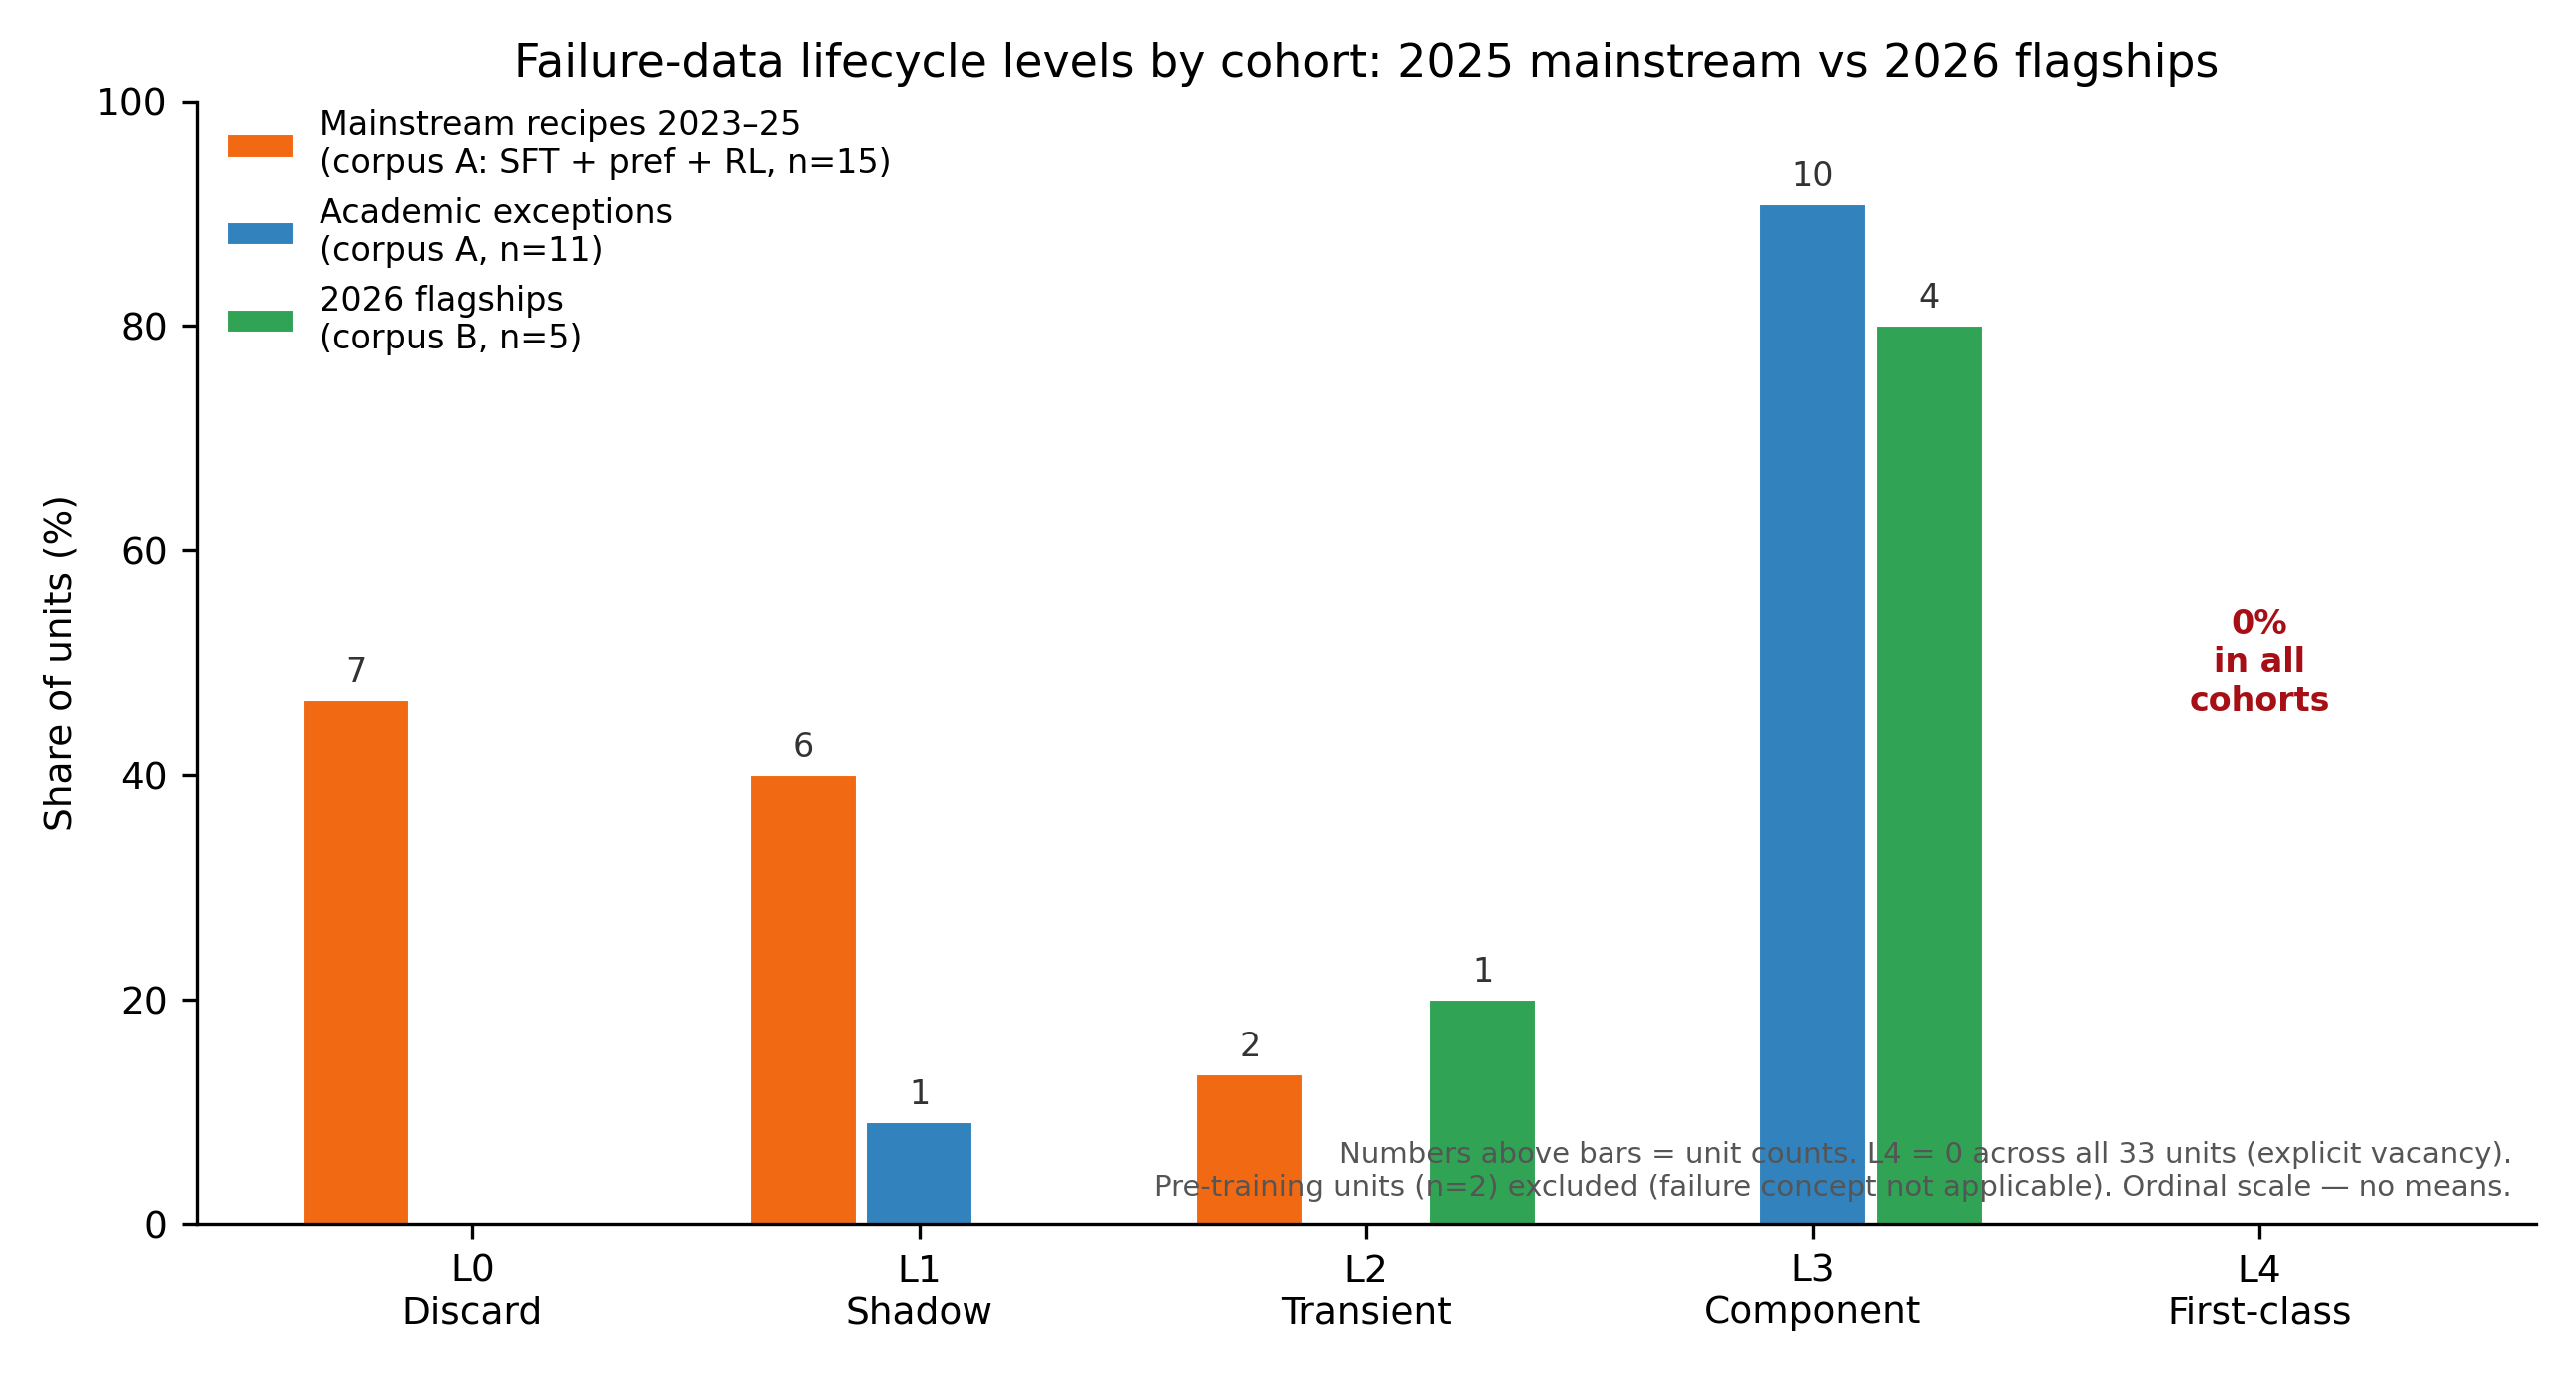
\includegraphics[width=0.95\textwidth]{fig2_level_distribution.png}
\caption{Distribution of failure-data lifecycle levels by cohort: mainstream recipes 2023--25 ($n{=}15$), academic exceptions ($n{=}11$), and 2026 flagships ($n{=}5$). Numbers above bars are unit counts; L4 $=$ 0 in all cohorts. Pre-training units excluded (failure concept not applicable). Ordinal scale---no means reported.}
\label{fig:levels}
\end{figure}

Table~\ref{tab:corpusA} and Figure~\ref{fig:levels} show a clean stratification by stage. \textbf{All seven SFT/distillation units are L0}: rejection-sampling-style discarding of failed trajectories is the default operation of 2023--25 SFT data production (R1, Llama 2/3, OpenR1-Math, Bespoke-Stratos, OpenMathReasoning, OpenMathInstruct-2). The preference stage is uniformly L1---six of six units, including MIPO, which grades negative-sample strength but performs no localization, attribution, or reflection, and is therefore best described as the upper bound of the shadow tier rather than a component design. The RL stage reaches L2; DAPO records multi-level L0+L2, with its all-failure-group removal constituting algorithm-level evidence of institutionalized discarding. Restricting to the mainstream subset (SFT + preference + RL, $n{=}15$): \textbf{0/15 units reach L3, and the subset's ordinal median is L1}. Every L3 unit sits in the academic-exception layer (10/11, with SPAR f26 coded at low confidence)---the community demonstrably knows how to build failure-rich datasets, and just as demonstrably does not ship them in mainstream recipes. Two boundary readings deserve note: the two evaluation-side L3 units evidence that localization- and attribution-type data exist, but for evaluation, not training---we code data form, not use equivalence (the OpenMathInstruct-2 boundary reading appears in Section~\ref{sec:codebook}).

\subsection{The pipeline layer: a generational shift, unnamed}

\begin{table}[t]
\centering
\caption{Corpus B (five 2026 flagships): lifecycle level $\times$ sub-dimensions ($n{=}5$).}
\label{tab:corpusB}
\resizebox{\textwidth}{!}{%
\begin{tabular}{lccccccccc}
\toprule
Model (release) & Main & Multi & Granularity & Attribution & Reflection & Domain & Openness & Vehicle & Conf. \\
\midrule
GPT-6 Astra (09-03) & \textbf{L2} & L0+L2 & trajectory & none & none & alignment & not-released & audit-loop & high\textsuperscript{\dag} \\
Claude Opus 5.5 (09-22) & \textbf{L3} & --- & trajectory & binary & none & alignment & not-released & audit-loop & medium \\
GLM-5.3 (2026 H2) & \textbf{L3} & L0+L3 & \textbf{step} & binary & none & capability & not-released & static-dataset & high \\
MiMo-V2.6 (09-22) & \textbf{L3} & --- & \textbf{step} & binary & \textbf{full-report} & alignment & not-released & static-dataset & high \\
DeepSeek-V4.1-Flash (09-09) & \textbf{L3} & --- & trajectory & \textbf{root-cause} & none & capability & not-released & RL-environment & high \\
\bottomrule
\end{tabular}}

\vspace{2pt}
\par\noindent{\footnotesize \textsuperscript{\dag}Unit confidence from the main-code mechanism (RL penalty, verbatim from the system card); monitoring/evaluation-routing mechanisms are medium (excerpt-level quotes).}
\end{table}

Table~\ref{tab:corpusB} locates each flagship. \textbf{Four of five units are L3; the cohort median is L3.} GPT-6 Astra is the sole sub-L3 flagship: its only training-side use of failure is a transient RL penalty---``penalize cheating and unauthorized actions'' \cite{openai2026gpt6}---while failure signals are explicitly routed to monitoring and evaluation (coded as L0 mechanisms under CR5, since the routing is stated). GLM-5.3 masks rather than deletes errors: ``Erroneous segments within trajectories are retained but masked out in the loss function, allowing the model to learn error correction behaviors'' \cite{zai2026glm5}, alongside notebook-style RL task selection against persistently-failed tasks and binary attribution separating model error from environment crash. MiMo-V2.6 is the only unit with all three elements, synthesizing training samples from real reward-hacking failures in a form that ``keeps the original error recognizable and makes the correction explicit'' \cite{xiaomi2026mimo}. DeepSeek-V4.1-Flash is structurally closest to L4: ``we collect negative feedback and model failure cases submitted by internal employees at scale,'' feeding ``systematic replay of failures and targeted RL against observed model weaknesses'' \cite{deepseek2026v41}---organized collection, root-cause attribution, and capability-domain scope. Claude Opus 5.5 drives training improvements from 7,200+ collected agent failure scenarios, but within the alignment domain only \cite{anthropic2026claude} (excerpt-level evidence; paraphrased here).

\begin{table}[t]
\centering
\caption{Sub-dimension distributions (unit level), Corpus A vs Corpus B.}
\label{tab:subdims}
\small
\begin{tabular}{llcc}
\toprule
Sub-dimension & Values & Corpus A ($n{=}28$) & Corpus B ($n{=}5$) \\
\midrule
Granularity & none / trajectory / step / causal / n.d. & 3 / 18 / 6 / \textbf{0} / 1 & 0 / 3 / 2 / \textbf{0} / 0 \\
Attribution & none / binary / root-cause / n.d. & 26 / \textbf{0} / 1 / 1 & 1 / 3 / 1 / 0 \\
Reflection & none / correction-pair / full-report / n.d. & 23 / 4 / \textbf{0} / 1 & 4 / 0 / \textbf{1} / 0 \\
Domain & capability / alignment / both / n.d. & 23 / 1 / 2 / 2 & 2 / 3 / 0 / 0 \\
Openness & released / not-released & \textbf{11 / 17} & \textbf{0 / 5} \\
Vehicle & none / pref-pair / static / RL-env / audit-loop & 9 / 8 / 9 / 2 / 0 & 0 / \textbf{0} / 2 / 1 / 2 \\
\bottomrule
\end{tabular}
\end{table}

Table~\ref{tab:subdims} shows the \emph{vehicle migration}, our second structural finding. In the 2025 mainstream cohort, 6/15 units carry failure via preference pairs; across the 14 mechanism records of the five flagships, \textbf{preference-pair carrying is 0} (audit-loop $\times$4, static-dataset $\times$5, RL-environment $\times$5). The same-vendor record is decisive on version dynamics: MIPO's graded negatives (L1) were retired in GLM 5.x, whose post-training chain contains no preference-optimization stage \cite{zai2025glm45,zai2026glm5}; and DeepSeek's own trajectory runs from R1's rejection sampling (2025-01, L0) to V4.1-Flash's failure replay (2026-09, L3), with the rejection-sampling stage gone \cite{deepseek2025r1,deepseek2026v41}.

\begin{table}[t]
\centering
\caption{Generational contrast: 2025 mainstream recipes vs 2026 flagships.}
\label{tab:generations}
\small
\begin{tabular}{lccccccccc}
\toprule
Cohort & $n$ & L0 & L1 & L2 & L3 & L4 & $\ge$L3 & Median \\
\midrule
2025 mainstream (SFT+pref+RL) & 15 & 7 (46.7\%) & 6 (40.0\%) & 2 (13.3\%) & 0 & 0 & \textbf{0 (0.0\%)} & L1 \\
2026 flagships & 5 & 0 & 0 & 1 (20\%) & 4 (80\%) & 0 & \textbf{4 (80.0\%)} & L3 \\
\bottomrule
\end{tabular}
\end{table}

Table~\ref{tab:generations} formalizes the shift; an exploratory Fisher exact test gives $p = .001$ (two-sided; identical one-sided). We stress the caveats: saturated purposive sampling, $n = 5$, ordinal data, no randomization---the distribution and the anchored quotes, not the test, carry the argument. Sensitivity checks bound the claim honestly: dropping low-confidence and boundary units leaves 0/14 at $\ge$L3 for the mainstream cohort and 3/4 for flagships (one-sided $p = .005$); adding pre-training units to the 2025 cohort changes nothing ($p < .001$); but comparing \emph{all} 28 Corpus-A units against the flagships yields 10/28 at $\ge$L3 and $p = .089$ (one-sided)---the generational contrast's strength depends on the ``mainstream recipe'' framing, since the academic-exception layer is by construction a counterexample layer. We therefore claim a generational shift in \emph{mainstream disclosed practice}, not a population estimate.

\subsection{The vacancy: three elements and openness}

\begin{table}[t]
\centering
\caption{Lifecycle level $\times$ three elements (all 33 units).}
\label{tab:elements}
\small
\begin{tabular}{lcccc}
\toprule
Level & $n$ & Locate (step/causal) & Attribute (binary/root-cause) & Reflect (pair/full-report) \\
\midrule
L0 & 9 & 0 & 0 & 0 \\
L1 & 7 & 0 & 0 & 0 \\
L2 & 3 & 0 & 0 & 0 \\
L3 & 14 & 8 (57.1\%) & 5 (35.7\%) & 5 (35.7\%) \\
L4 & 0 & --- & --- & --- \\
\bottomrule
\end{tabular}
\end{table}

Table~\ref{tab:elements} shows that the three elements co-vary with level---strictly concentrated in L3 (e.g., localization 8/14 vs 0/19 elsewhere; exploratory Fisher $p = .00022$; attribution and reflection 5/14 vs 0/19, $p = .008$)---but are jointly satisfied by \textbf{exactly one unit of 33 (MiMo-V2.6)}, and even within L3 by one of fourteen. The elements remain individually scarce: causal-granularity localization is absent corpus-wide (0/33); root-cause attribution exists in one evaluation-side unit in Corpus A (PRMBench) and one flagship (DeepSeek); full reflective reports exist in one unit (MiMo). Openness splits the corpus along an institutional fault line: the 11 units whose failure data is released are \emph{all} on the academic side (10 academic exceptions plus HH-RLHF's released rejected sides), while the flagships release none (0/5)---MiMo's publication of five reward-hacking failure trajectories is exemplar-level disclosure, and its open-sourcing of roughly 7,000 RL environments is not a release of failure data.

The L4 scan across both corpora returns \textbf{0/33}, with the four criteria failing in a structured way: criterion (i), the three elements, is met only by MiMo; criterion (ii), scale, is undisclosed for MiMo; criterion (iii), explicit theorization as methodology, is met by no vendor---DeepSeek frames the entire apparatus as engineering: ``the marginal return of engineering the data and environment pipeline substantially exceeds that of algorithmic novelty'' \cite{deepseek2026v41}; and criterion (iv), public release, is met by no flagship. The nearest misses are LEMA (elements largely present and released, but at $10^4$ scale and outside mainstream recipes) and DeepSeek-V4.1-Flash (organized scale and root-cause attribution, but unnamed and unreleased). Finally, the procedural corroboration: the August--October 2026 arXiv re-check surfaced no large-scale failure-dataset or industrial failure-reflection methodology paper; adjacent hits concern failure detection \cite{zhang2026foresight}.

\section{Discussion}\label{sec:discussion}

\subsection{A vacancy that is a finding}

The L4 tier was expected to be empty when the codebook was written, and the audit confirms it systematically. The situation is therefore not ``failure data does not work''---the methodological families supply controlled positive evidence (Section~\ref{sec:background})---nor ``nobody wants it'': a senior policy figure named it publicly in July 2026 \cite{waic2026}, and four of five flagship pipelines now contain failure components. Within the audited disclosure layer and the 2026-10-13 evidence window, first-class failure data is an \emph{unoccupied high ground}: proven at small scale, named in public discourse, demanded by the weakest model dimensions, and claimed by no one as methodology. The vacancy is falsifiable and time-stamped: a public release within twelve months that satisfies all four L4 criteria would refute it, and we propose exactly that as a monitoring indicator.

\subsection{The best vehicle may be environments, not datasets}

The vehicle migration (Table~\ref{tab:subdims}) suggests the field has voted with its infrastructure. The preference-pair vehicle---the shadow form---did not survive its era: MIPO, its most systematic design, was retired rather than scaled \cite{zai2025glm45}. The three flagship carriers each embody one element: MiMo's reflection-revision data carries reflection, DeepSeek's replay environments carry attribution-driven targeting, GLM's masked segments carry localization. It is plausible that the terminal form of failure data is not a static annotated corpus but a \emph{closed loop}---collect, attribute, replay, retrain---as DeepSeek's disclosures imply \cite{deepseek2026v41}. We hold a dual position. For industry pipelines, environments plus replay may indeed dominate: they keep failure data on-policy and current. But closed loops are private by construction; if the community is ever to study failure-data methodology cumulatively, static, openly licensed, tripartite-annotated corpora remain the only shareable form---and PRS demonstrates that reflective \emph{text} data, trainable with a plain SFT loss, already works \cite{hao2026prs}. Both forms, and a bridge between them, belong in the roadmap.

\subsection{Implications for the weakest dimensions}

Our audit measures practice, not effects, and we resist causal inference beyond the evidence. The alignment of incentives is nonetheless notable: generalization and calibration, where current training is weakest, are precisely where failure data is a candidate signal, by the posterior-contraction argument of Section~\ref{sec:intro-arg}. RLVR appears to sharpen pass@1 without expanding pass@$k$ \cite{yue2025rlvr}; hallucination behaves as a calibration failure reinforced by confident-guessing rewards \cite{kalai2025halluc}; post-training measurably damages confidence calibration \cite{he2023calibration,xie2026know}. Training on attributed failures is, formally, training on the \emph{boundary of competence}---the region where a well-calibrated model must decline. The strongest existing hint is PRS's double-unseen result (12.00 vs 0.00) \cite{hao2026prs}; establishing the generalization--calibration payoff of failure data at scale is an open experimental program, which our roadmap's evaluation component is designed to seed.

\subsection{Verifier dependence}\label{sec:verifier}

Failure data inherits its definition from verifiers, and verifiers can be gamed. Reward hacking is a \emph{fake success}---toxic to train on as either positive or negative without causal attribution. The flagships' components are largely answers to exactly this problem: MiMo's online grader jointly inspects successful and failed rollouts and zeroes the reward of confirmed-hacked passes, converting them to failures \cite{xiaomi2026mimo}; GLM closes reward shortcuts in solver trajectories and separates model error from environment collapse \cite{zai2026glm5}; DeepSeek records hacking and environment crashes as failure trajectories fed back to the RL framework \cite{deepseek2026v41}. The open problem is the no-verifier domain: where success cannot be checked automatically, failure attribution requires new instruments, without which the methodology cannot leave verifiable domains such as mathematics and code.

\subsection{Limitations}\label{sec:limitations}

Five limitations bound our claims. (1) \emph{Disclosure bias, both directions}: undisclosed failure practice would make our L-levels underestimates; vendor embellishment would make components overstated. All conclusions are therefore scoped to disclosed practice, and we release the anchoring quotes so readers can re-adjudicate. (2) \emph{Single coder}: the audit is one coder's application of a public codebook; the intra-rater $\kappa$ is pending (Section~\ref{sec:method}), and no inter-rater reliability exists. (3) \emph{Ordinal discipline}: L0--L4 supports medians and distributions only; we report no means or interval statistics. (4) \emph{Time truncation}: the corpus is an autumn-2026 snapshot of a moving target; units are version-anchored, and the generational contrast is cohort-framed (the full-corpus sensitivity at $p = .089$ marks the boundary of the statistical claim). (5) \emph{Quote confidence}: verbatim quotes anchor all high-confidence Corpus-B codes; three Corpus-B mechanisms and most Corpus-A anchors rest on excerpt-level evidence, which we paraphrase rather than quote.

\section{Roadmap: Making Failure Data a First-Class Citizen}\label{sec:roadmap}

The audit's vendor mapping (Table~\ref{tab:roadmap}) shows which components exist and which are missing; none of the five vendors assembles them all, and the open-corpus component is vacant across the entire industry.

\begin{table}[t]
\centering
\caption{Roadmap components $\times$ flagship coverage (from the audit's sub-dimension records).}
\label{tab:roadmap}
\footnotesize
\setlength{\tabcolsep}{3.5pt}
\begin{tabular}{p{3.2cm}p{2.4cm}p{2.4cm}p{2.4cm}p{1.9cm}p{1.9cm}}
\toprule
Component & MiMo & DeepSeek & GLM-5.3 & Claude & GPT-6 \\
\midrule
(a) Tripartite collection/annotation protocol & partial (reflection-revision samples, hacking domain only) & partial (employee submission + classification, no reflective text) & partial (masked retention, no reflection) & none & none \\
(b) Toxicity cleaning \& causal attribution & yes (hacked passes zeroed; infrastructure failures removed) & yes (hacking/crash recorded as failures) & partial (binary model-vs-environment removal) & partial (flawed-environment attribution) & not disclosed \\
(c) Verifier-dependence handling & yes (joint success/failure grading) & partial (inspection agent flags) & yes (reward shortcuts closed) & not disclosed & not disclosed \\
(d) Open corpus \& shared protocols & none (open environments $\neq$ open failure data) & none & none & none & none \\
\bottomrule
\end{tabular}
\end{table}

From this mapping we specify the missing infrastructure:

\begin{enumerate}
\item \textbf{Tripartite data schema.} Failure records as first-class objects with three mandatory fields---error type (localized at step or causal granularity), root cause, and correction text---together with provenance (task, policy version, verifier verdict). The schema is vehicle-neutral: it applies to static datasets, preference-pair extensions, and environment logs.
\item \textbf{Collection and annotation protocols.} Who collects failures (users, employees, rollouts), how they are sampled for diversity rather than volume, and which analyzer annotates them---with the analyzer model disclosed, a detail our verification chain shows to be load-bearing \cite{hao2026prs}.
\item \textbf{Toxicity cleaning and causal attribution.} A mandatory pre-training stage that separates fake successes (reward hacking) from infrastructure failures from valuable model failures, following the flagship precedents (Section~\ref{sec:verifier}).
\item \textbf{Verifier-dependence handling.} Protocols for dual-grading passed-but-suspect trajectories, and a research program for failure attribution in no-verifier domains.
\item \textbf{Open corpus and shared protocols.} The ecosystem's single large-scale release retaining failures is OpenR1-Math-Raw ($\sim$10\textsuperscript{6} raw trajectories, L3 with openness=released but elements incomplete) \cite{openr12025mathraw}; we propose community tripartite annotation layers over exactly such raw seeds, with licenses and provenance conventions---activity that no vendor currently undertakes (Table~\ref{tab:roadmap}d).
\item \textbf{An evaluation benchmark.} Controlled comparisons of models trained with and without matched failure data, scored on out-of-distribution generalization (double-unseen designs, following \cite{hao2026prs}) and on calibration (confidence--correctness alignment), plus ``failure literacy'' tasks measuring localization and attribution (extending \cite{zheng2024processbench,song2025prmbench}).
\end{enumerate}

Falsifiable predictions follow from the audit: no L4 release within twelve months would extend the vacancy; a continued preference-pair share near zero would confirm the vehicle migration; and the first vendor to theorize its failure pipeline as methodology would occupy the vacant tier.

\section{Conclusion}\label{sec:conclusion}

We audited how LLM training practice treats failure data, and found a structured paradox. The methodology is proven at small scale and the discourse has named it, yet across 33 audited units the highest lifecycle tier is empty (0/33), the 2023--25 mainstream never rose above transient failure gradients (0/15 at $\ge$L3; all SFT units pure discard), and the 2026 flagships---which do operate failure components (4/5 at L3)---keep them local, unnamed, and unreleased, having already abandoned the preference-pair vehicle that once carried failure implicitly (0/14 flagship mechanisms). Success gives direction; failure gives precision; current practice, within everything it discloses, throws the precision away. The audit instruments---a lifecycle codebook, a boundary-case registry, and open coding records---are released with this paper so that the vacancy can be monitored, and refuted, in public.

\section*{Data and Materials Availability}

The codebook (five-level lifecycle criteria plus six sub-dimensions), the 14-case boundary registry, the mechanism-level coding table (44 records with anchoring quotes, section anchors, source tiers, and confidence ratings), the reproduction script (\texttt{coding\_data.py}), and both figures are packaged as supplementary materials accompanying this paper. % TODO(user): replace with permanent repository URL/DOI (GitHub + Zenodo recommended) before submission.

\section*{Code Availability}

The reproduction script and the coding dataset (CSV) are released with the supplementary materials under an open license. % TODO(user): confirm license (e.g., MIT for code, CC-BY 4.0 for data) and repository URL.

\section*{Funding}

This work received no external funding. % TODO(user): confirm.

\section*{Conflict of Interest}

The author is affiliated with Yu Yugui Strategy Lab, an independent research institution; there are no financial or personal relationships with the vendors audited that could influence this work. % TODO(user): confirm wording.

\section*{AI-Assistance Disclosure}

This research was conducted and this manuscript was prepared with the assistance of large language model systems used as research and writing collaborators (literature search, coding-table organization, and drafting). All evidence units, coding decisions, quotations, and numbers were selected, verified, and take responsibility for by the human author, following the verification gates described in Section~4.3; the audit's two upstream propagating errors were caught and corrected by exactly this gate. This disclosure is voluntary; arXiv policy holds authors responsible for all content and sanctions unchecked AI-generated material.

\bibliographystyle{unsrtnat}
\bibliography{references}

\end{document}
